\fancyhead[LE]{\fontsize{8.5pt}{10pt}\selectfont\textbf{\textsf{\thepage}}\quad \textbf{\textsf{CHƯƠNG 1}}\quad \textsf{Các hàm số và Mô hình}}
\fancyhead[RO]{\fontsize{8.5pt}{10pt}\selectfont\textsf{MỤC 1.3}\quad \textsf{Các hàm số mới từ các hàm số cũ}\quad \textbf{\textsf{\thepage}}}

\noindent
\begin{minipage}[t]{0.265\textwidth}
    \fontsize{8pt}{10.2pt}\selectfont
    \vspace*{2.45cm}
    
    \centering
    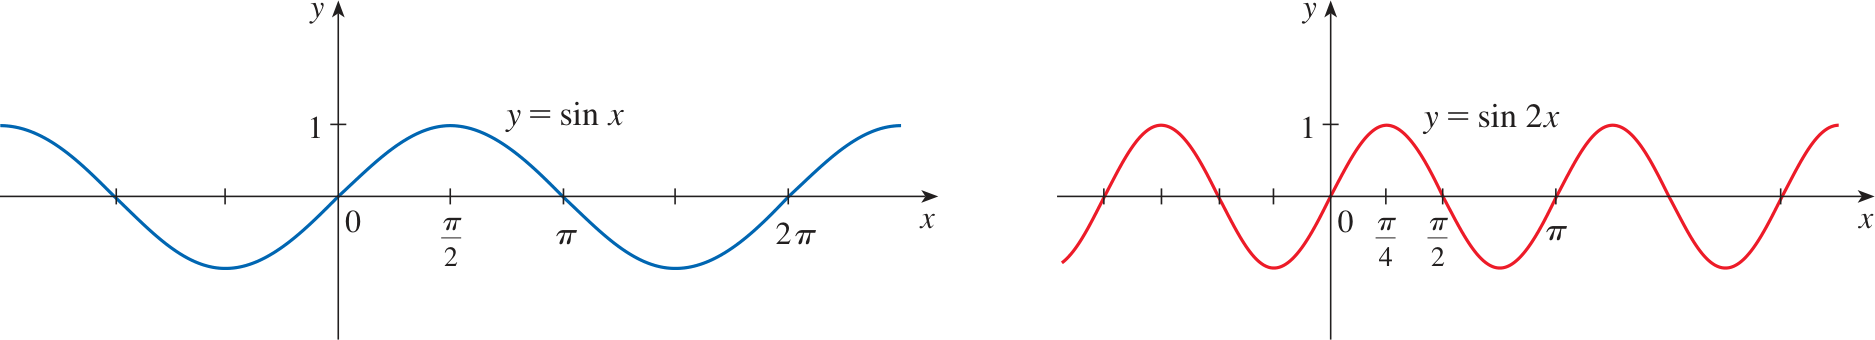
\includegraphics[width=0.92\linewidth]{images/p0074_fig6.png}
    \vspace{2pt}
    
    \raggedright
    \textbf{\textsf{HÌNH 6}}
    
    \vspace{4.2cm}
    \textbf{\textsf{HÌNH 8}}
    
    \vspace{2.4cm}
    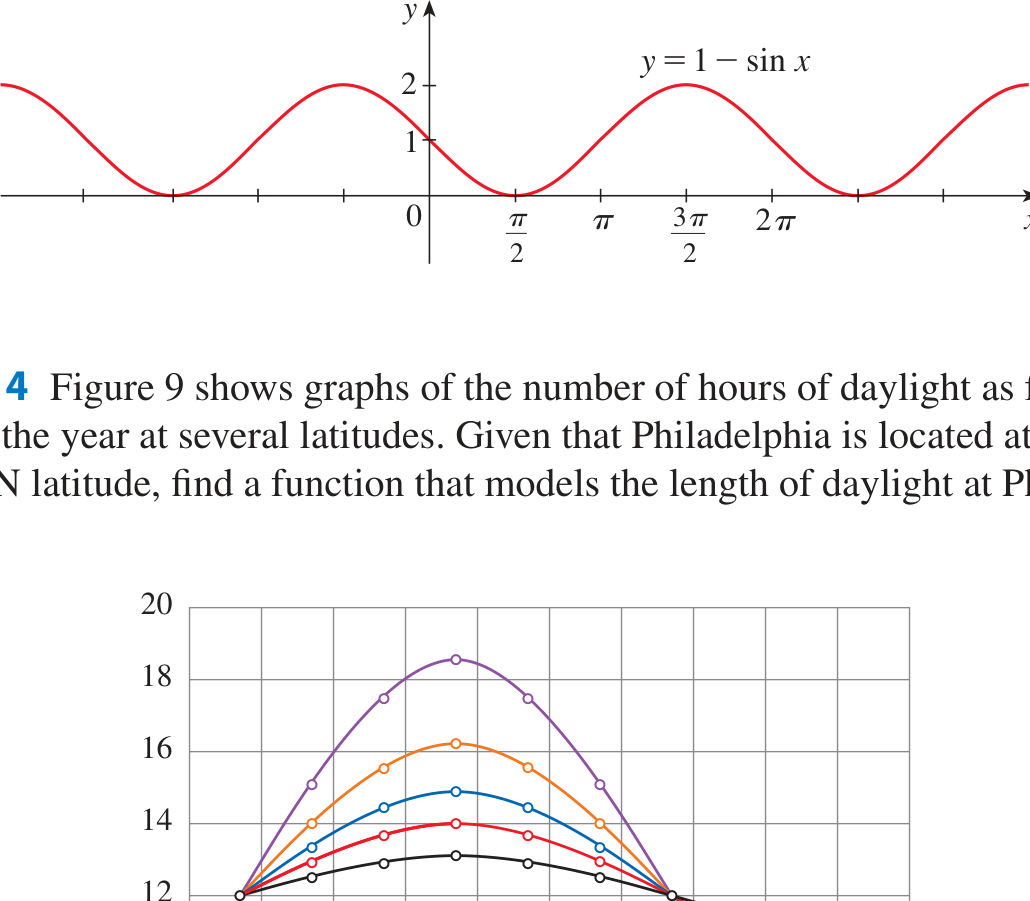
\includegraphics[width=0.92\linewidth]{images/p0074_fig9.png}
    \vspace{3pt}
    
    \textbf{\textsf{HÌNH 9}}\par
    {\fontsize{7.2pt}{9pt}\selectfont
    Đồ thị độ dài thời gian ban ngày từ ngày 21 tháng 3 đến ngày 21 tháng 12 tại các vĩ độ khác nhau\par
    \vspace{2pt}
    \textit{Nguồn:} Phỏng theo L. Harrison, \textit{Daylight, Twilight, Darkness and Time} (New York: Silver, Burdett, 1935), 40.\par}
\end{minipage}%
\hfill
\begin{minipage}[t]{0.708\textwidth}
    \fontsize{9.3pt}{13.2pt}\selectfont
    \textbf{\textsf{\color{stewartcyan}VÍ DỤ 3}}\quad Phác thảo đồ thị của mỗi hàm số sau:
    \begin{enumerate*}[label=(\alph*), itemjoin=\qquad]
        \item $y = \sin 2x$
        \item $y = 1 - \sin x$
    \end{enumerate*}

    \vspace{0.15cm}
    \noindent\textbf{\textsf{\color{stewartcyan}LỜI GIẢI}}
    
    \noindent(a) Ta nhận được đồ thị của hàm số $y = \sin 2x$ từ đồ thị của $y = \sin x$ bằng cách co theo phương ngang với hệ số $2$. (Xem Hình 6 và Hình 7.) Vì chu kỳ của hàm số $y = \sin x$ là $2\pi$, nên chu kỳ của $y = \sin 2x$ là $2\pi/2 = \pi$.

    \begin{center}
    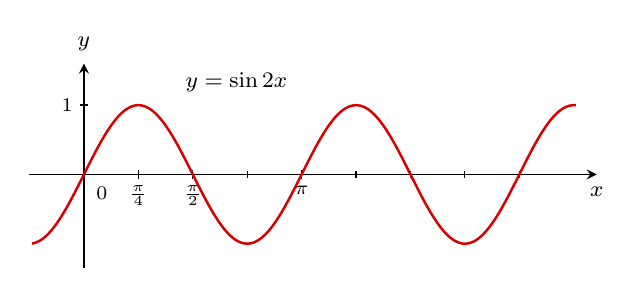
\begin{tikzpicture}[x=0.88cm, y=0.88cm, baseline=(current bounding box.center)]
        % Trục tọa độ
        \draw[->, >=stealth, line width=0.6pt] (-0.8, 0) -- (7.4, 0) node[below=1pt, font=\fontsize{8pt}{9pt}\selectfont] {$x$};
        \draw[->, >=stealth, line width=0.6pt] (0, -1.35) -- (0, 1.6) node[above=1pt, font=\fontsize{8pt}{9pt}\selectfont] {$y$};
        
        % Vạch chia trục tung
        \draw[line width=0.5pt] (-0.06, 1) -- (0.06, 1) node[left=2pt, font=\fontsize{7.5pt}{9pt}\selectfont] {$1$};
        \node[below right=1pt, font=\fontsize{7.5pt}{9pt}\selectfont] at (0,0) {$0$};
        
        % Vạch chia trục hoành
        \draw[line width=0.5pt] ({pi/4}, -0.06) -- ({pi/4}, 0.06) node[below=2pt, font=\fontsize{7pt}{8pt}\selectfont] {$\frac{\pi}{4}$};
        \draw[line width=0.5pt] ({pi/2}, -0.06) -- ({pi/2}, 0.06) node[below=2pt, font=\fontsize{7pt}{8pt}\selectfont] {$\frac{\pi}{2}$};
        \draw[line width=0.5pt] ({pi}, -0.06) -- ({pi}, 0.06) node[below=2pt, font=\fontsize{7pt}{8pt}\selectfont] {$\pi$};
        
        % Vạch phụ
        \draw[line width=0.4pt] ({3*pi/4}, -0.05) -- ({3*pi/4}, 0.05);
        \draw[line width=0.4pt] ({5*pi/4}, -0.05) -- ({5*pi/4}, 0.05);
        \draw[line width=0.4pt] ({3*pi/2}, -0.05) -- ({3*pi/2}, 0.05);
        \draw[line width=0.4pt] ({7*pi/4}, -0.05) -- ({7*pi/4}, 0.05);
        \draw[line width=0.4pt] ({2*pi}, -0.05) -- ({2*pi}, 0.05);
        
        % Đồ thị y = sin(2x)
        \draw[line width=0.9pt, red!85!black, domain=-0.75:7.1, samples=150, smooth] 
            plot (\x, {sin(2*\x r)});
            
        % Tên đồ thị
        \node[above, font=\fontsize{8pt}{9pt}\selectfont] at (2.2, 1.05) {$y = \sin 2x$};
    \end{tikzpicture}
    
    \vspace{1pt}
    {\centering\textbf{\textsf{HÌNH 7}}\par}
    \end{center}

    \noindent(b) Để có được đồ thị của hàm số $y = 1 - \sin x$, ta lại bắt đầu từ đồ thị của $y = \sin x$. Ta lấy đối xứng qua trục $x$ để nhận được đồ thị của $y = -\sin x$, rồi sau đó tịnh tiến lên trên 1 đơn vị để được đồ thị của $y = 1 - \sin x$. (Xem Hình 8.)

    \begin{center}
    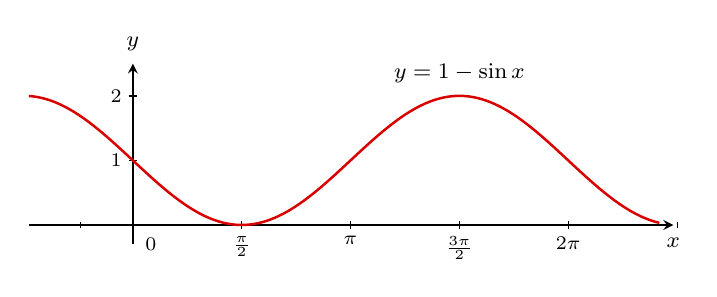
\begin{tikzpicture}[x=0.88cm, y=0.82cm, baseline=(current bounding box.center)]
        % Trục tọa độ
        \draw[->, >=stealth, line width=0.6pt] (-1.5, 0) -- (7.8, 0) node[below=1pt, font=\fontsize{8pt}{9pt}\selectfont] {$x$};
        \draw[->, >=stealth, line width=0.6pt] (0, -0.3) -- (0, 2.5) node[above=1pt, font=\fontsize{8pt}{9pt}\selectfont] {$y$};
        
        % Vạch chia trục tung
        \draw[line width=0.5pt] (-0.06, 1) -- (0.06, 1) node[left=2pt, font=\fontsize{7.5pt}{9pt}\selectfont] {$1$};
        \draw[line width=0.5pt] (-0.06, 2) -- (0.06, 2) node[left=2pt, font=\fontsize{7.5pt}{9pt}\selectfont] {$2$};
        \node[below right=1pt, font=\fontsize{7.5pt}{9pt}\selectfont] at (0,0) {$0$};
        
        % Vạch chia trục hoành
        \draw[line width=0.5pt] ({pi/2}, -0.06) -- ({pi/2}, 0.06) node[below=2pt, font=\fontsize{7pt}{8pt}\selectfont] {$\frac{\pi}{2}$};
        \draw[line width=0.5pt] ({pi}, -0.06) -- ({pi}, 0.06) node[below=2pt, font=\fontsize{7pt}{8pt}\selectfont] {$\pi$};
        \draw[line width=0.5pt] ({3*pi/2}, -0.06) -- ({3*pi/2}, 0.06) node[below=2pt, font=\fontsize{7pt}{8pt}\selectfont] {$\frac{3\pi}{2}$};
        \draw[line width=0.5pt] ({2*pi}, -0.06) -- ({2*pi}, 0.06) node[below=2pt, font=\fontsize{7pt}{8pt}\selectfont] {$2\pi$};
        
        % Vạch phụ
        \draw[line width=0.4pt] (-0.75, -0.05) -- (-0.75, 0.05);
        \draw[line width=0.4pt] ({5*pi/2}, -0.05) -- ({5*pi/2}, 0.05);
        
        % Đồ thị y = 1 - sin(x)
        \draw[line width=0.9pt, red!85!black, domain=-1.5:7.6, samples=150, smooth] 
            plot (\x, {1 - sin(\x r)});
            
        % Tên đồ thị
        \node[above, font=\fontsize{8pt}{9pt}\selectfont] at ({3*pi/2}, 2.05) {$y = 1 - \sin x$};
    \end{tikzpicture}\hfill{\color{stewartcyan}$\blacksquare$}
    \end{center}

    \vspace{0.1cm}
    \noindent\textbf{\textsf{\color{stewartcyan}VÍ DỤ 4}}\quad Hình 9 cho thấy các đồ thị biểu diễn số giờ ban ngày như là các hàm số theo thời gian trong năm tại một số vĩ độ khác nhau. Biết rằng thành phố Philadelphia nằm ở vĩ độ khoảng $40^\circ\text{B}$ (vĩ độ Bắc), hãy tìm một hàm số mô hình hóa độ dài thời gian ban ngày tại Philadelphia.

    \begin{center}
    \begin{tikzpicture}[x=0.78cm, y=0.23cm]
        % Lưới tọa độ
        \draw[line width=0.35pt, gray!45] (0,0) grid[xstep=1, ystep=2] (9,20);
        \draw[line width=0.6pt, gray!75] (0,0) rectangle (9,20);
        
        % Vạch chia trục tung (Giờ)
        \foreach \y in {0, 2, 4, 6, 8, 10, 12, 14, 16, 18, 20} {
            \node[left=3pt, font=\fontsize{7.5pt}{8.5pt}\selectfont] at (0, \y) {\y};
        }
        \node[left=18pt, font=\fontsize{8pt}{9pt}\selectfont] at (0, 10) {Giờ};
        
        % Các tháng trên trục hoành
        \node[below=3pt, font=\fontsize{6.8pt}{7.8pt}\selectfont] at (0,0) {Th.3};
        \node[below=3pt, font=\fontsize{6.8pt}{7.8pt}\selectfont] at (1,0) {Th.4};
        \node[below=3pt, font=\fontsize{6.8pt}{7.8pt}\selectfont] at (2,0) {Th.5};
        \node[below=3pt, font=\fontsize{6.8pt}{7.8pt}\selectfont] at (3,0) {Th.6};
        \node[below=3pt, font=\fontsize{6.8pt}{7.8pt}\selectfont] at (4,0) {Th.7};
        \node[below=3pt, font=\fontsize{6.8pt}{7.8pt}\selectfont] at (5,0) {Th.8};
        \node[below=3pt, font=\fontsize{6.8pt}{7.8pt}\selectfont] at (6,0) {Th.9};
        \node[below=3pt, font=\fontsize{6.8pt}{7.8pt}\selectfont] at (7,0) {Th.10};
        \node[below=3pt, font=\fontsize{6.8pt}{7.8pt}\selectfont] at (8,0) {Th.11};
        \node[below=3pt, font=\fontsize{6.8pt}{7.8pt}\selectfont] at (9,0) {Th.12};
        
        % Màu các đường cong
        \definecolor{lat60}{RGB}{186, 130, 195}
        \definecolor{lat50}{RGB}{235, 140, 60}
        \definecolor{lat40}{RGB}{0, 160, 220}
        \definecolor{lat30}{RGB}{230, 90, 75}
        \definecolor{lat20}{RGB}{80, 80, 80}
        
        % Vẽ các đường cong: y = 12 + A * sin(pi * x / 6)
        \draw[line width=0.75pt, lat60, smooth] plot[domain=0:9, samples=50] (\x, {12 + 6.75*sin(\x * 30)});
        \draw[line width=0.75pt, lat50, smooth] plot[domain=0:9, samples=50] (\x, {12 + 4.30*sin(\x * 30)});
        \draw[line width=0.75pt, lat40, smooth] plot[domain=0:9, samples=50] (\x, {12 + 3.00*sin(\x * 30)});
        \draw[line width=0.75pt, lat30, smooth] plot[domain=0:9, samples=50] (\x, {12 + 2.05*sin(\x * 30)});
        \draw[line width=0.75pt, lat20, smooth] plot[domain=0:9, samples=50] (\x, {12 + 1.25*sin(\x * 30)});
        
        % Các điểm tròn trên từng đường cong
        \foreach \x in {0, 1, ..., 9} {
            \filldraw[fill=white, draw=lat60, line width=0.45pt] (\x, {12 + 6.75*sin(\x * 30)}) circle (1.2pt);
            \filldraw[fill=white, draw=lat50, line width=0.45pt] (\x, {12 + 4.30*sin(\x * 30)}) circle (1.2pt);
            \filldraw[fill=white, draw=lat40, line width=0.45pt] (\x, {12 + 3.00*sin(\x * 30)}) circle (1.2pt);
            \filldraw[fill=white, draw=lat30, line width=0.45pt] (\x, {12 + 2.05*sin(\x * 30)}) circle (1.2pt);
            \filldraw[fill=white, draw=lat20, line width=0.45pt] (\x, {12 + 1.25*sin(\x * 30)}) circle (1.2pt);
        }
        
        % Nhãn các vĩ độ bên phải
        \draw[line width=0.4pt, gray!60] (9, {12 - 1.25}) -- (9.3, 10.75);
        \node[right=2pt, font=\fontsize{7.2pt}{8.2pt}\selectfont] at (9.3, 10.75) {$20^\circ\text{ B}$};
        
        \draw[line width=0.4pt, gray!60] (9, {12 - 2.05}) -- (9.3, 9.95);
        \node[right=2pt, font=\fontsize{7.2pt}{8.2pt}\selectfont] at (9.3, 9.95) {$30^\circ\text{ B}$};
        
        \draw[line width=0.4pt, gray!60] (9, {12 - 3.00}) -- (9.3, 9.00);
        \node[right=2pt, font=\fontsize{7.2pt}{8.2pt}\selectfont] at (9.3, 9.00) {$40^\circ\text{ B}$};
        
        \draw[line width=0.4pt, gray!60] (9, {12 - 4.30}) -- (9.3, 7.70);
        \node[right=2pt, font=\fontsize{7.2pt}{8.2pt}\selectfont] at (9.3, 7.70) {$50^\circ\text{ B}$};
        
        \draw[line width=0.4pt, gray!60] (9, {12 - 6.75}) -- (9.3, 5.25);
        \node[right=2pt, font=\fontsize{7.2pt}{8.2pt}\selectfont] at (9.3, 5.25) {$60^\circ\text{ B}$};
    \end{tikzpicture}
    \end{center}
\end{minipage}